% b3_ml_dl — Block 3: Learning. ML half + datasets: Member 4. DL half: Amin.
% Numbers come from experiments/ml/results.json and real_results.json (seed 42); figures from
% `python -m er_agent.learning.ml.figures`. Needs \usepackage{graphicx}.
\section{Block 3 --- Learning: risk prediction}

\noindent\textit{Educational simulation only. No real medical diagnosis or treatment recommendation.}

\subsection{Datasets}

Both datasets are synthetic, seeded and regenerable with
\texttt{python -m er\_agent.learning.data\_gen --seed 42}.

\paragraph{Tabular dataset (8\,000 patients).}
A latent severity $s\sim\mathrm{Gamma}(1.3, 0.42)$ drives every vital sign (heart rate, systolic/diastolic
pressure, SpO$_2$, temperature, respiratory rate), plus independent Gaussian noise, so features are correlated
but class distributions overlap. Symptoms (chest pain, shortness of breath, fever, abdominal pain) and
confusion are drawn with probabilities that increase with $s$. The label is computed from an early-warning
score inspired by NEWS2: point bands on the five vitals, $+3$ for confusion, $+1$/$+2$ for age $\geq65$/$\geq80$,
and symptom bonuses (chest pain $+2$, shortness of breath $+1$, both together $+1$ more). A small Gaussian
``clinician judgement'' term is added and the score is cut into Low / Medium / High / Critical.
Two choices keep the problem from being trivially learnable:
(i)~6.5\% label noise, 80\% of it moved to an adjacent class;
(ii)~a realistic imbalance of 48.5 / 32.9 / 13.2 / 5.4\%.
Two pure-noise columns are added on purpose to test feature selection.
On the brief's patients the generator gives P1~$\to$~Critical, P2~$\to$~Medium (exactly on the cut-point) and
P3~$\to$~Low.

\paragraph{Temporal dataset (4\,000 sequences, for the DL models).}
Sequences of 5--12 steps over (hr, sbp, spo2, temp, rr), zero-padded at the end with a mask. Each follows one
of five severity paths: stable, noisy-stable, slow deterioration, fast (accelerating) deterioration, recovery.
The label depends on the trajectory, not only on the last step: the last step's warning score is projected two
steps ahead using the recent slope. 400 explicit \emph{pairs} share identical last-step vitals but have
opposite trends. In 88\% of pairs the two labels differ, so a model that only sees the last step cannot be
right on both. This is the key experiment for ML vs.\ DL.

\subsection{Preprocessing and feature selection}

Stratified 70/15/15 train/validation/test split (seed 42). A single \texttt{sklearn} \texttt{Pipeline} handles
everything:
\begin{itemize}
  \item median imputation and standardisation for numeric columns;
  \item most-frequent imputation and one-hot encoding for categorical columns;
  \item the classifier.
\end{itemize}
The pipeline is saved with \texttt{joblib}, so the agent never re-implements preprocessing, and missing fields
at inference time are imputed (with a logged warning).

A feature is kept only if both its mutual information (train) and its permutation importance (validation,
$\Delta$ macro-F1) are higher than those of every pure-noise column (Fig.~\ref{fig:ml-fi}). The Random Forest's
impurity importance is shown for comparison but not used: it gives the two noise columns ($\approx0.05$) more
importance than real but rare binary signals such as confusion ($0.016$), a known bias towards continuous
features. Kept: age, hr, sbp, spo2, temp, rr, chest pain, shortness of breath, fever, consciousness. Dropped:
the noise columns, abdominal pain (weak by construction), and diastolic pressure, which is redundant with
systolic (permutation importance $\approx0$ despite a Spearman correlation of $-0.38$).

\begin{figure}[h]
  \centering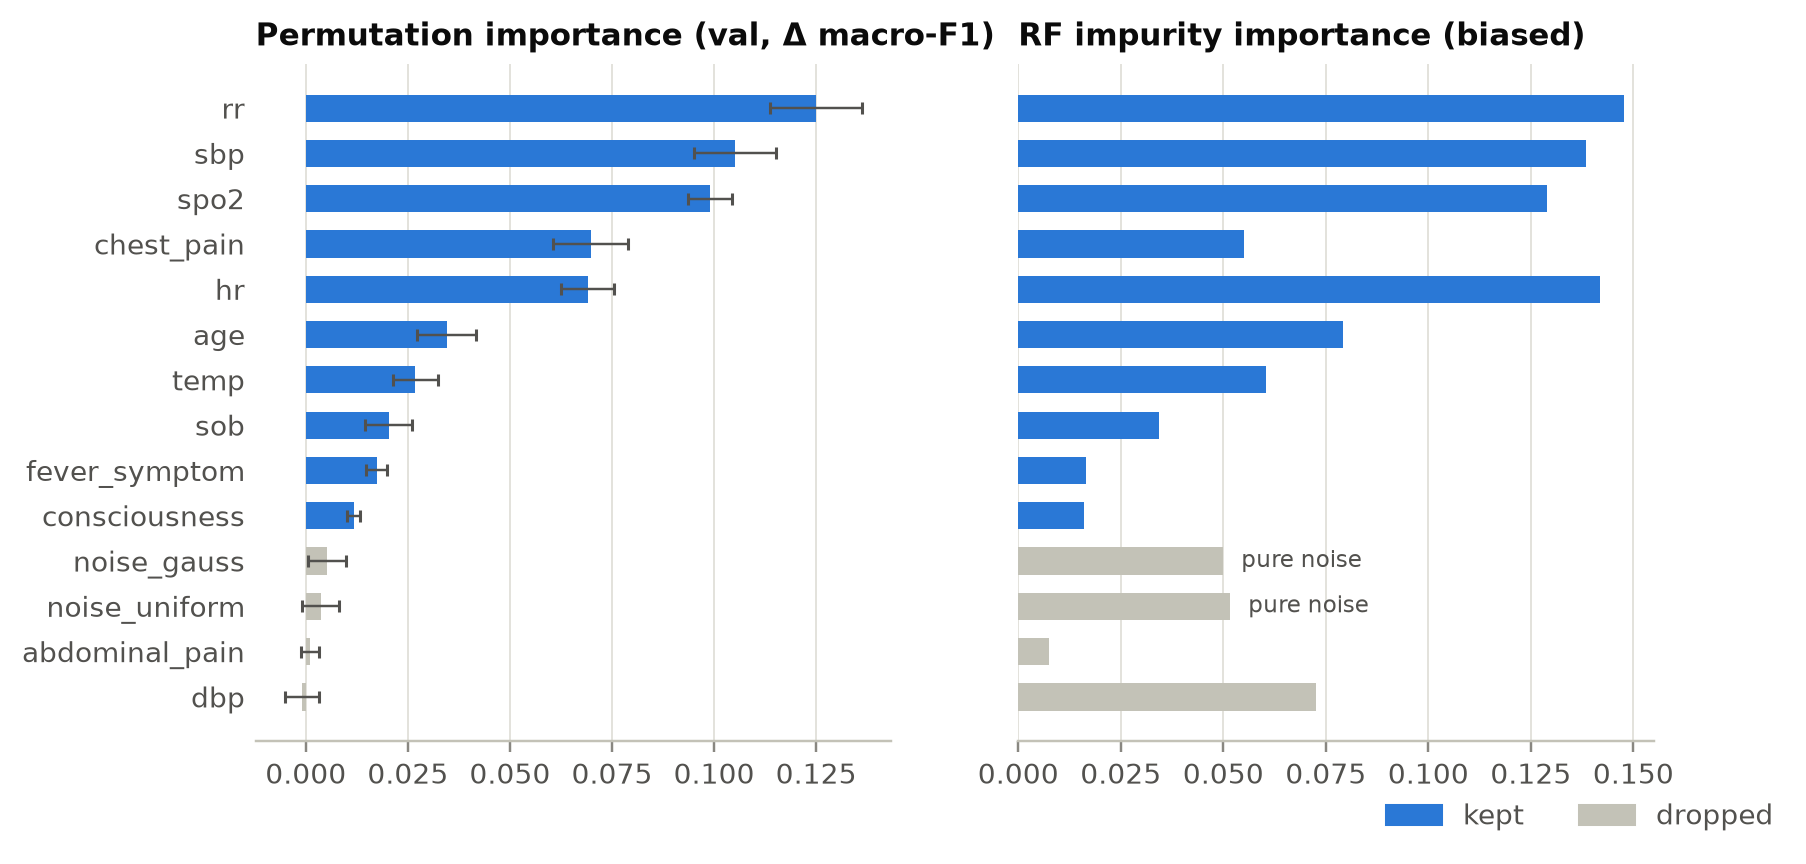
\includegraphics[width=\linewidth]{figures/ml_feature_importance.png}
  \caption{Feature selection. Gray = dropped. Impurity importance (right) ranks pure noise above real
  symptoms.}
  \label{fig:ml-fi}
\end{figure}

\subsection{Models}

Four classifiers, each trained with and without \texttt{class\_weight="balanced"}:
\begin{itemize}
  \item \textbf{Decision Tree} (depth 6): interpretable, and can be compared with the logic engine's rules;
  \item \textbf{Random Forest}: non-linear, robust, gives feature importances;
  \item \textbf{Logistic Regression}: linear baseline with naturally calibrated probabilities;
  \item \textbf{Histogram Gradient Boosting}: strong tabular baseline.
\end{itemize}
The Random Forest was then tuned with a 5-fold \texttt{GridSearchCV} (54 candidates, macro-F1). Best:
300 trees, depth 14, at least 3 patients per leaf, $\sqrt{d}$ features tried per split, and
\texttt{balanced\_subsample} class weights; CV macro-F1 0.735.

\begin{figure}[h]
  \centering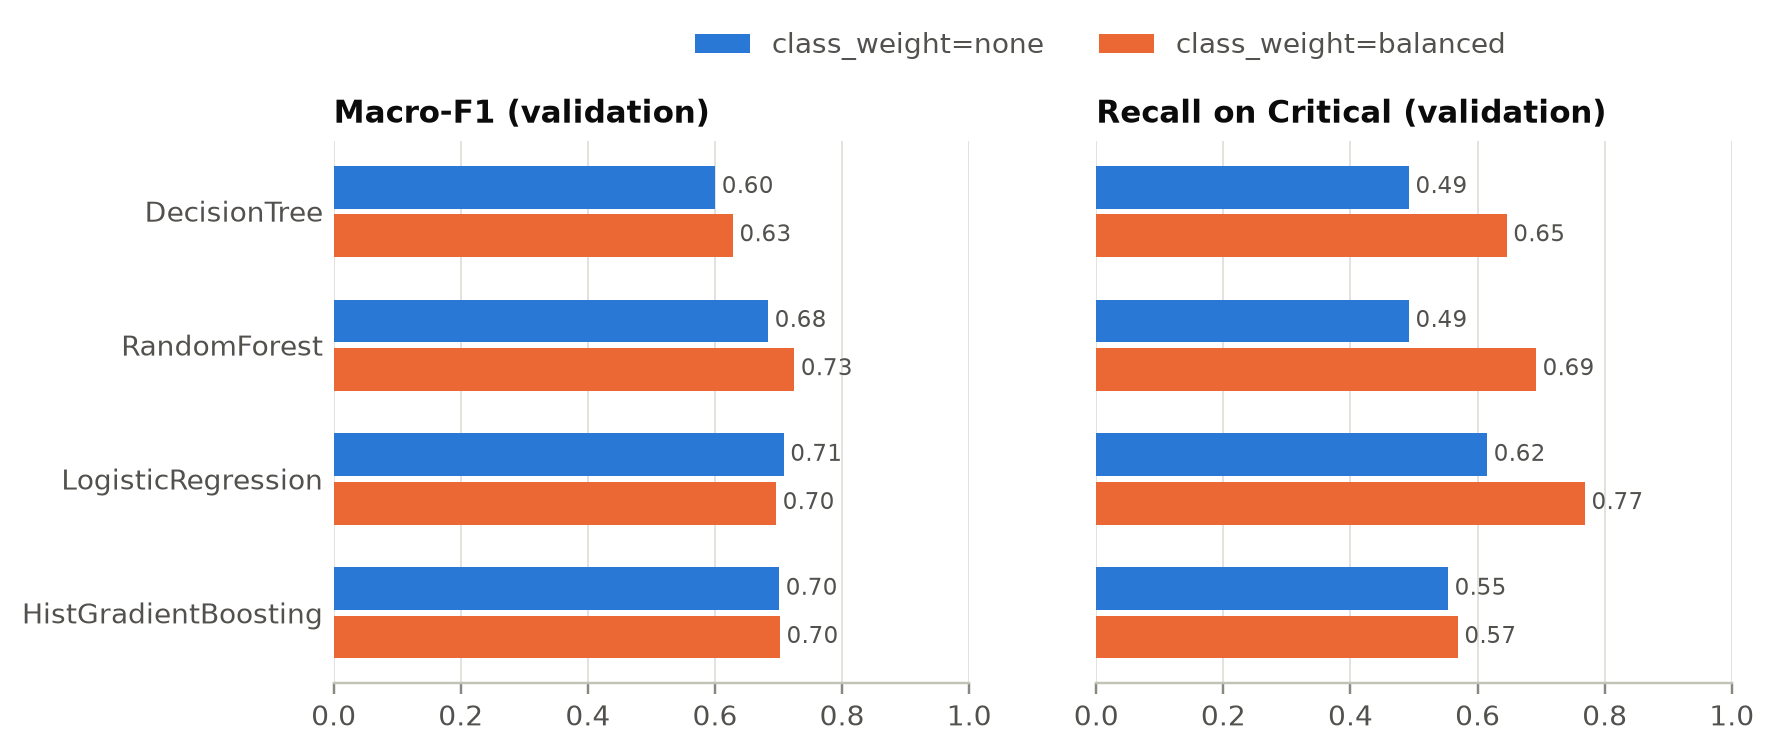
\includegraphics[width=\linewidth]{figures/ml_model_comparison.png}
  \caption{Validation macro-F1 and recall on the Critical class.}
  \label{fig:ml-models}
\end{figure}

Class weighting has little effect on macro-F1 but raises recall on Critical sharply: from 0.49 to 0.69 for the
RF, and from 0.62 to 0.77 for logistic regression (Fig.~\ref{fig:ml-models}). In triage, missing a critical
patient costs far more than over-triaging one, so balanced weighting is used.

\paragraph{Calibration.}
The knowledge base fires rules on thresholds such as $p\geq0.7$, so the probability must mean what it says.
The tuned RF is under-confident: in Fig.~\ref{fig:ml-cal} its curve lies above the diagonal, i.e.\ it is
right more often than it claims (ECE 0.078 on validation). Sigmoid and isotonic calibration
(\texttt{CalibratedClassifierCV}, 5-fold) bring ECE to 0.025 and 0.028. Isotonic was chosen because it costs
no macro-F1 (0.729 vs.\ 0.731, while sigmoid drops to 0.716).

\begin{figure}[h]
  \centering
  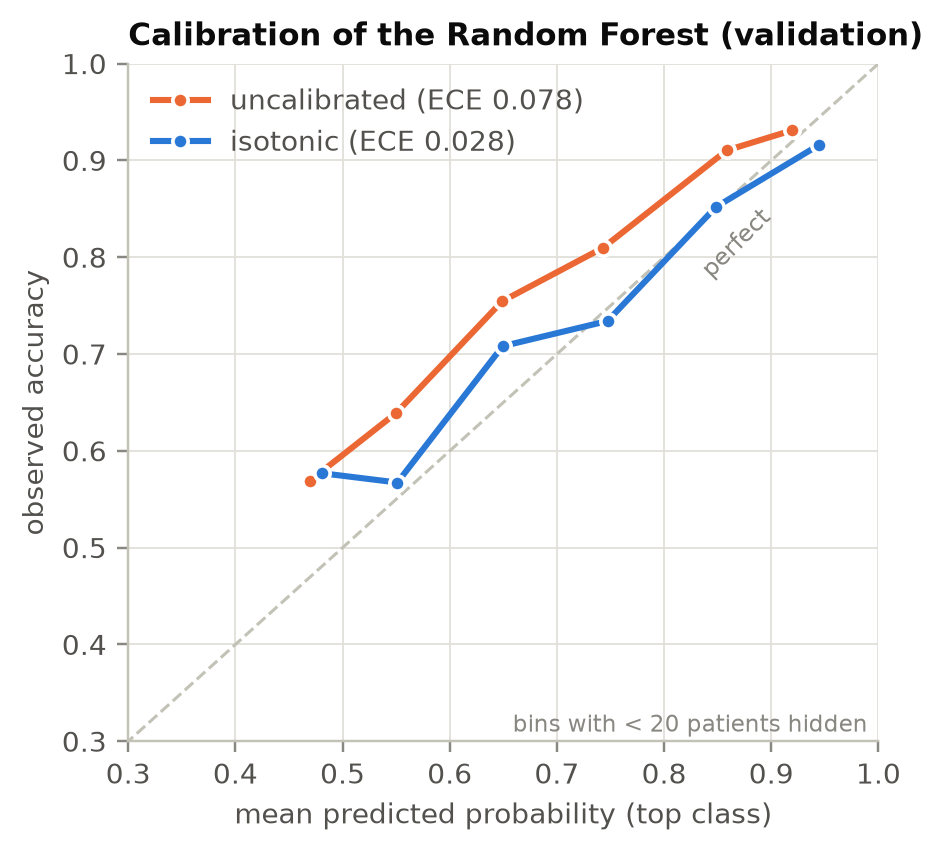
\includegraphics[width=0.48\linewidth]{figures/ml_reliability.png}\hfill
  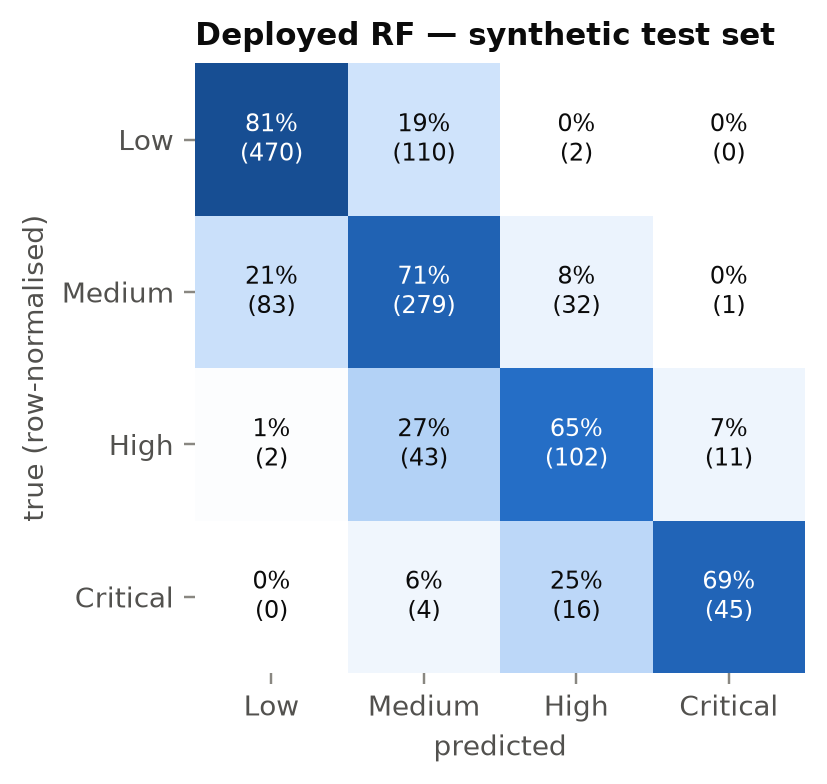
\includegraphics[width=0.46\linewidth]{figures/ml_confusion.png}
  \caption{Left: reliability diagram before and after calibration. Right: deployed model on the test set.}
  \label{fig:ml-cal}
\end{figure}

\paragraph{Deployed model and test results.}
Calibrated (isotonic) Random Forest, evaluated once on the 1\,200 held-out test patients (saved as
\texttt{models/ml\_rf.joblib}):

\begin{center}
\begin{tabular}{lcccc}
\hline
 & Low & Medium & High & Critical \\ \hline
recall & 0.81 & 0.71 & 0.65 & 0.69 \\
F1     & 0.83 & 0.67 & 0.66 & 0.74 \\ \hline
\end{tabular}
\end{center}

\noindent Accuracy 0.747, macro-F1 0.723, ECE 0.031. The confusion matrix is almost entirely on and next to
the diagonal: errors are between adjacent levels, consistent with the adjacent-class label noise.

\paragraph{Integration.}
\texttt{predict\_ml(patient)} takes a Contract-6 patient and returns \texttt{(label, p)}; the agent inserts
\texttt{("ML\_Risk", pid, label, p)}. On the brief's example:
\begin{itemize}
  \item P1 $\to$ (Critical, 0.99);
  \item P3 $\to$ (Low, 0.96);
  \item P2 $\to$ (Low, 0.55), with Medium at 0.43;
  \item P4 (\texttt{dynamic\_icu\_lost}) $\to$ Critical;
  \item P2 after the vitals updates of \texttt{dynamic\_deterioration} moves to High/Critical.
\end{itemize}
P2 lies exactly on our Low/Medium cut-point. The expected ``Medium'' is the \emph{fused} risk derived by the
logic engine, which combines this weak ML signal with fever and the DL trend.

\subsection{Bonus: from the decision tree to learned rules in the KB}

The ML model enters the knowledge base as one opaque fact, \texttt{ML\_Risk(x, label, p)}. To link the learned
and symbolic parts more directly, we turned a decision tree into Horn rules the logic engine can reason with,
trace and explain like its hand-written ones.\footnote{Generated by
\texttt{python -m er\_agent.learning.ml.rules\_export}.}

\paragraph{Method.}
\begin{enumerate}
  \item Each patient is discretized into the same facts the world model emits, using the shared thresholds
  (\texttt{world/thresholds.py}): \texttt{LowOxygen}, \texttt{Tachycardia}, \texttt{LowBloodPressure},
  \texttt{Fever}, \texttt{Elderly}, \texttt{Tachypnea}, \texttt{HasSymptom(x, s)}.
  \item One shallow tree (depth 5, balanced class weights) is trained per target:
  \texttt{HighRisk(x)} $\Leftrightarrow$ label $\in$ \{High, Critical\}, and
  \texttt{CriticalRisk(x)} $\Leftrightarrow$ label = Critical.
  \item Each leaf predicting the target becomes a rule whose premises are the conditions on its path.
  Horn clauses cannot express ``fact absent'', so negative conditions are \emph{dropped}. This makes the
  rule more general, so it is re-validated on held-out data.
  \item A rule is kept only if its validation precision is $\geq0.7$, the same confidence threshold the KB
  applies to \texttt{ML\_Risk}/\texttt{DL\_Risk}, its 95\% Wilson lower bound is $\geq0.6$, and it covers at
  least 20 patients. Rules subsumed by a more general kept rule are removed.
\end{enumerate}

The lower bound matters. Without it, two \texttt{CriticalRisk} rules passed with 0.72--0.73 precision on
validation and fell to 0.47--0.63 on test: when choosing among many candidates with small support, some are
just lucky.

\paragraph{Result.} Five rules, all holding on the untouched test split (SoB = ShortnessOfBreath):

\begin{center}
\resizebox{\linewidth}{!}{%
\begin{tabular}{lcc}
\hline
rule & val.\ precision [95\% low] & test precision \\ \hline
\texttt{Learned\_R1}: HasSymptom(x, ChestPain) $\land$ Tachycardia(x) $\to$ HighRisk(x) & 0.87 [0.73] & 0.87 \\
\texttt{Learned\_R2}: HasSymptom(x, SoB) $\land$ Tachycardia(x) $\to$ HighRisk(x) & 0.86 [0.74] & 0.82 \\
\texttt{Learned\_R3}: Tachypnea(x) $\to$ HighRisk(x) & 0.86 [0.76] & 0.85 \\
\texttt{Learned\_R4}: LowBloodPressure(x) $\to$ HighRisk(x) & 0.82 [0.71] & 0.78 \\
\texttt{Learned\_R5}: HasSymptom(x, ChestPain) $\land$ HasSymptom(x, SoB) $\to$ HighRisk(x) & 0.82 [0.68] & 0.80 \\ \hline
\end{tabular}}
\end{center}

\noindent Compared with the hand-written rules on the same test patients (forward chaining to a fixpoint):
\begin{itemize}
  \item hand-written R1, R2 derive \texttt{HighRisk} with precision 0.92 but recall only 0.15;
  \item the learned rules reach recall 0.67 at precision 0.74;
  \item the two sets agree: \texttt{Learned\_R4} (low blood pressure) generalises the hand-written R1
  (chest pain $\land$ low blood pressure).
\end{itemize}
\textbf{No \texttt{CriticalRisk} rule passes the filter, at any tree depth.} From present/absent facts alone, a
Critical patient cannot be singled out reliably by a short rule; that needs the graded information in the
probabilities. So \texttt{CriticalRisk} stays derived from \texttt{DL\_Risk}/\texttt{ML\_Risk} (R5) and the
hand-written R6, and the learned rules only feed \texttt{HighRisk}. On P1 of the brief, all five learned rules
fire; none fires for P2 or P3. On the real KTAS data the learned rules keep 0.62 precision but reach only 0.20
recall, the same distribution gap as in the next subsection.
The rules ship as \texttt{er\_agent/learning/ml/learned\_rules.json}; a test regenerates them and fails if the
shipped file is stale.

\subsection{Bonus: evaluation on real triage data}

To test how realistic our generator is, we used a public real dataset: 1\,267 adult emergency-department
visits from two Korean hospitals, each with a reference triage level on the Korean Triage and Acuity Scale
(KTAS, 1--5) set by expert reviewers (Moon et al., \textit{PLOS ONE} 14(9):e0216972, 2019, supporting
information S1, CC BY 4.0). Expert KTAS was mapped to our classes as 1~$\to$~Critical, 2~$\to$~High,
3~$\to$~Medium, 4/5~$\to$~Low, giving 2.1 / 17.4 / 38.4 / 42.2\%.

The dataset has the same vitals as ours and adds the triage nurse's own KTAS and the hospital outcome. SpO$_2$
is missing for 55\% of visits, so a missing-value indicator was added for the ``full'' feature set. We also use
the hospital outcome (admitted to a ward or ICU, or died: 30.8\%) as an \emph{external} check, since no model
was trained on it. The results are in Fig.~\ref{fig:ml-real}; all CIs are 95\% bootstrap intervals over
patients.

\begin{figure}[h]
  \centering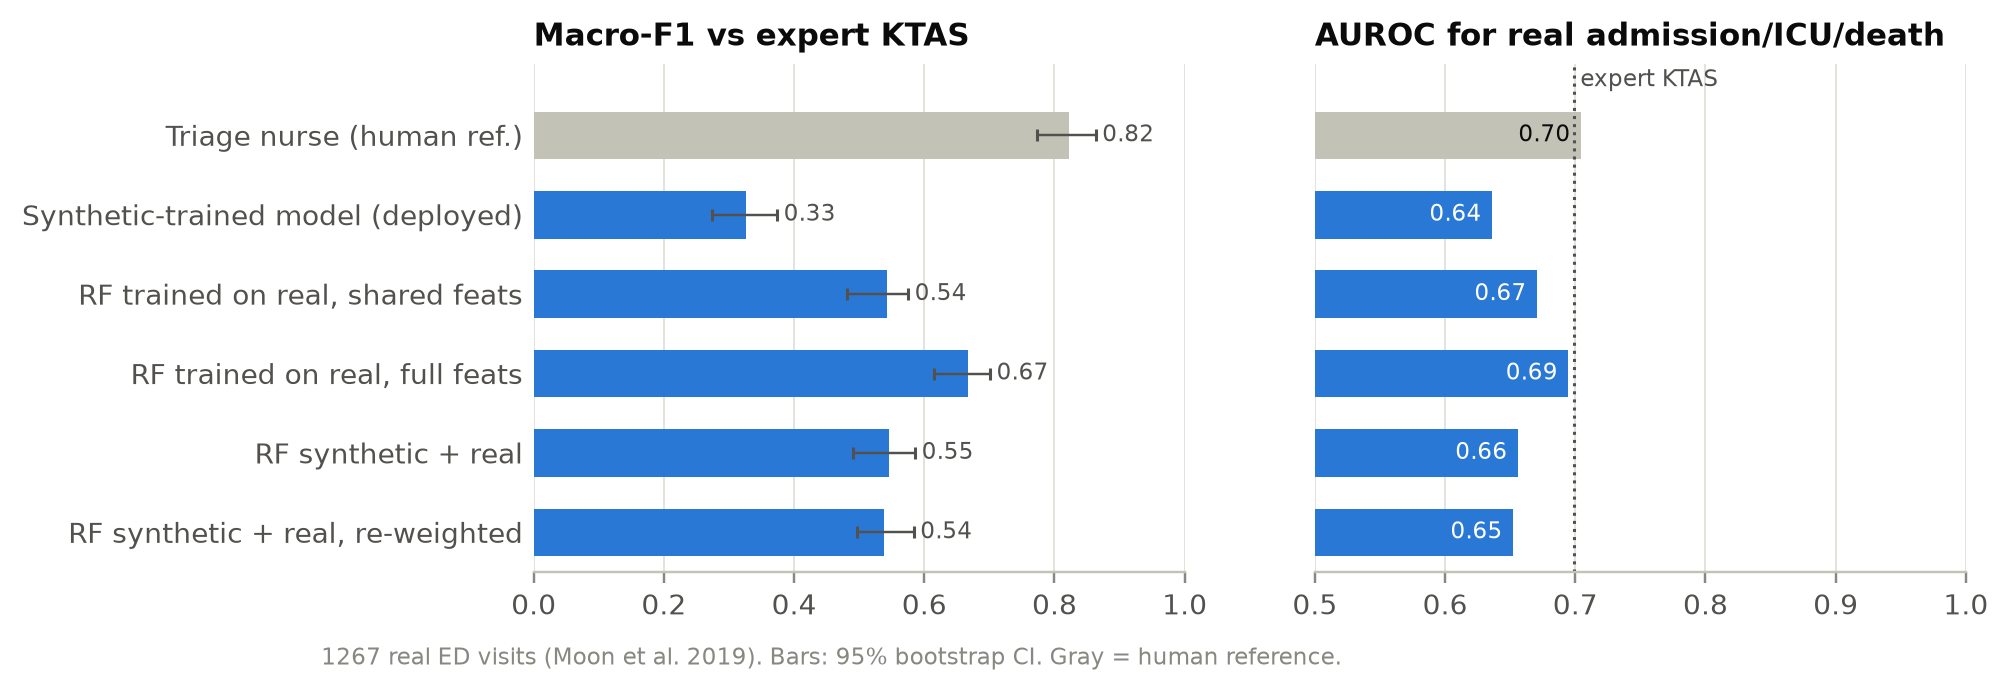
\includegraphics[width=\linewidth]{figures/ml_real_transfer.png}
  \caption{Real KTAS data. Rows A/C use 3$\times$ repeated stratified 5-fold CV. Dotted line: AUROC of the
  expert KTAS itself.}
  \label{fig:ml-real}
\end{figure}

\paragraph{Synthetic to real: the model does not transfer.}
Applied unchanged, the deployed model reaches only 0.33 macro-F1 [0.27, 0.37]. It under-triages systematically: it
labels 76\% of real Medium patients as Low, and 22 of the 26 real Critical patients (85\%) lower than Critical. Figure~\ref{fig:ml-gap} shows why. On real
patients our label rule still ranks severity in the right order (Spearman 0.39), but the real classes are
compressed: the median score of a real Critical patient is 6, against 13 in our synthetic data. Real
emergencies are often recognised before vital signs become extreme.

\begin{figure}[h]
  \centering
  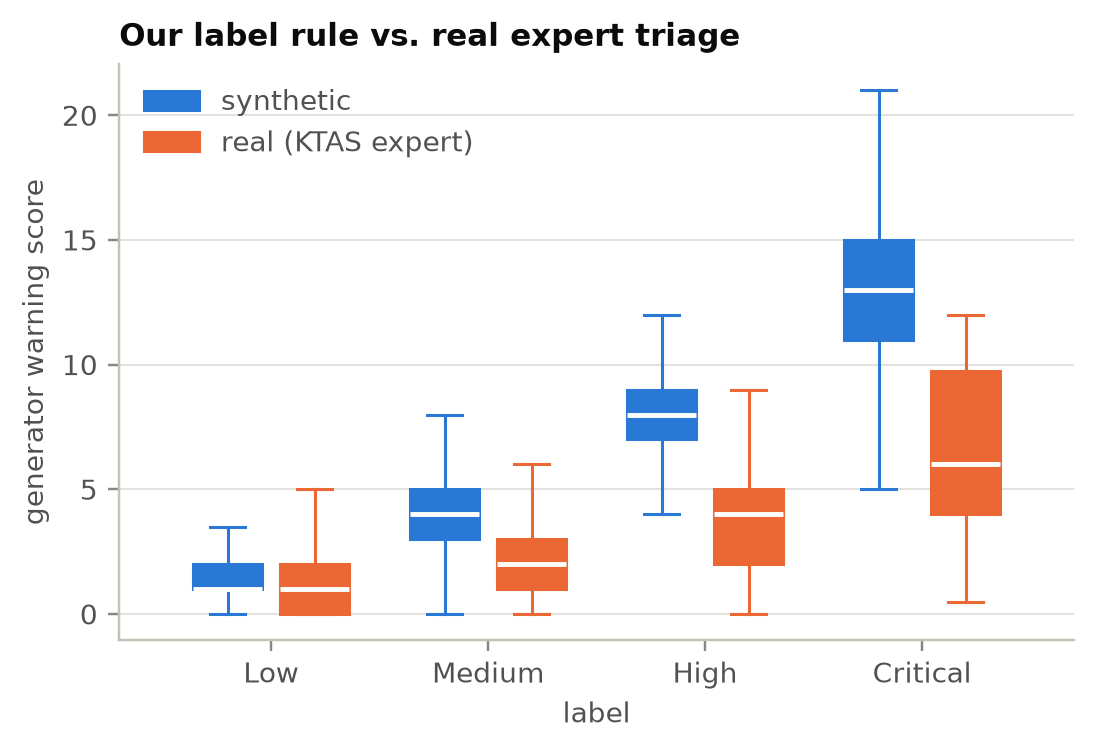
\includegraphics[width=0.52\linewidth]{figures/ml_real_generator_score.png}\hfill
  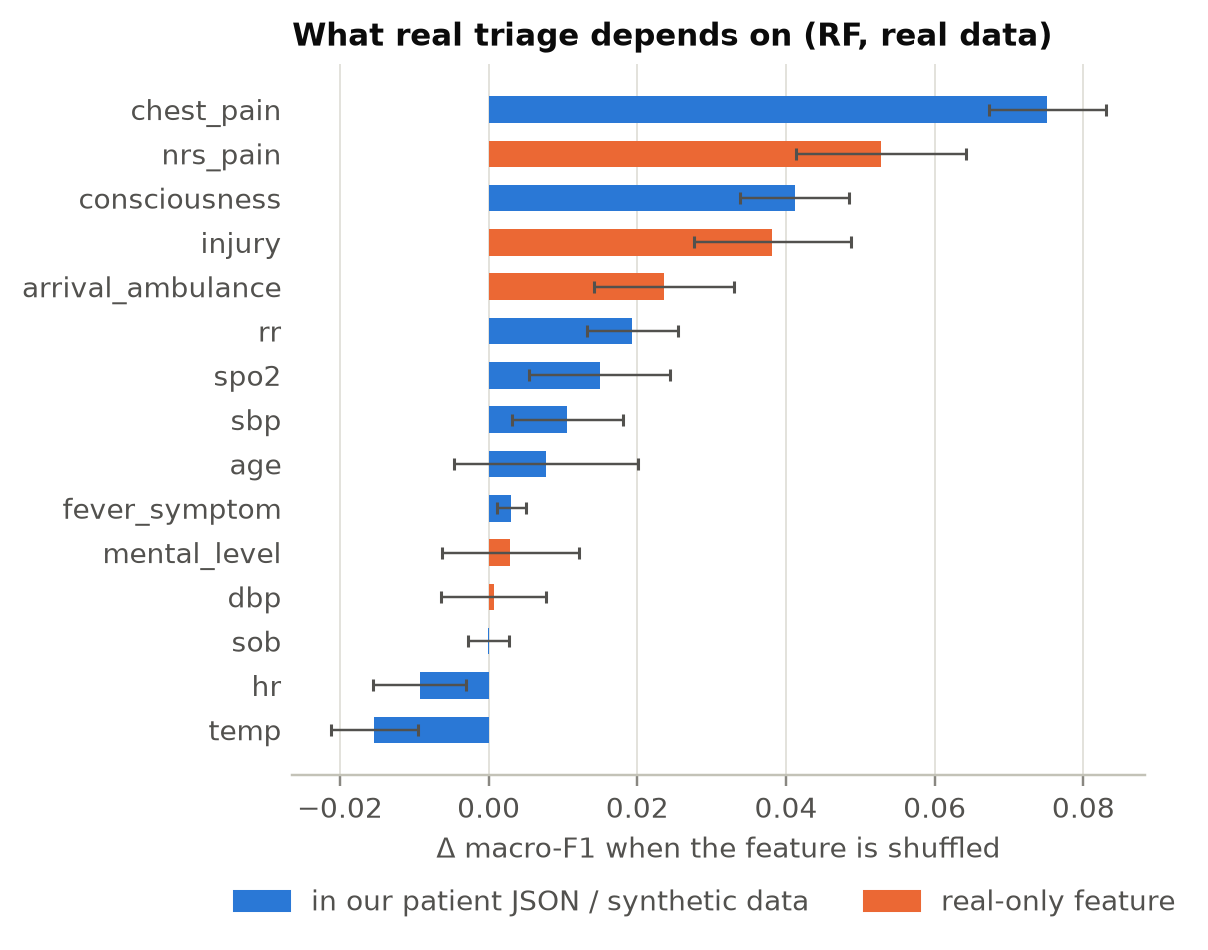
\includegraphics[width=0.46\linewidth]{figures/ml_real_importance.png}
  \caption{Left: our generator's warning score per class, synthetic vs.\ real. Right: permutation importance of
  an RF trained on real data (orange = information our patient JSON does not carry).}
  \label{fig:ml-gap}
\end{figure}

\paragraph{Real to real.}
Trained and cross-validated on the real data, the same pipeline gives:
\begin{itemize}
  \item 0.54 macro-F1 [0.48, 0.58] with our ten features;
  \item 0.67 [0.61, 0.70] once real-only information is added (pain score, injury, ambulance arrival,
  consciousness level), with Critical recall 0.78 [0.59, 0.92].
\end{itemize}
The importance plot shows real triage is driven by chest pain, pain intensity, consciousness and injury
(Fig.~\ref{fig:ml-gap}, right). Heart rate and temperature contribute nothing once those are known, the opposite
of our generator, where vitals dominate. For predicting admission, ICU or death, this model's AUROC (0.70) is
on par with the expert KTAS itself (0.70) and with the nurse (0.70).

\paragraph{Mixing synthetic and real data.}
Adding our 8\,000 synthetic rows to each real training fold does not help: 0.55 [0.49, 0.59] macro-F1, and 0.54
when re-weighted so both sources count equally, against 0.54 with real data only. The synthetic distribution is
too far from the real one to act as useful pre-training.

\paragraph{Human reference.}
The triage nurses agree with the experts at 0.82 macro-F1, but miss 42\% of Critical cases. This is an
optimistic reference: the experts' labels come from reviewing the nurses' own triage records, and nurses see
much more than ten features.

\subsection{Limitations}

\begin{itemize}
  \item \textbf{Synthetic data.} The deployed model learns our generator's rule, not medicine. The real-data
  experiment shows it does not transfer (0.33 macro-F1 on real patients): its Critical class needs far more
  extreme vitals than real Critical patients have, and it ignores pain, injury and arrival mode, which real
  triage depends on.
  \item \textbf{Label noise and the ceiling.} With 6.5\% injected noise plus the judgement term, about 75\%
  accuracy is near the best achievable; errors are almost all between adjacent levels.
  \item \textbf{Imbalance.} Critical is 5.4\% of the training data (65 test patients) and 2.1\% of the real
  data (26 patients). Critical recall is therefore uncertain: the real-data CIs span about 0.3.
  \item \textbf{Overfitting.} The RF reaches 0.89 macro-F1 on train vs.\ 0.72 on test. This is expected with
  depth-14 trees on noisy labels; validation and test agree (0.73 / 0.72), so model selection did not
  overfit the validation set.
  \item \textbf{Calibration is only as good as the distribution.} ECE is 0.03 on synthetic test data, but 0.32
  on the real data: the probabilities the KB thresholds rely on are only meaningful in-distribution.
  \item \textbf{Single snapshot.} The tabular model sees one moment in time; trends are the DL model's job
  (next subsection).
  \item \textbf{Real-data caveats.} Our mapping of 5 KTAS levels to 4 classes is one choice among several;
  symptoms were extracted from free-text chief complaints with simple keyword rules; SpO$_2$ is missing for
  55\% of visits.
\end{itemize}

\subsection{Deep learning on vitals history}
% TODO(Amin): GRU / LSTM on data/temporal.npz, last-step baseline, paired-trajectory experiment.

\subsection{Roles of ML and DL in the agent}
% Joint paragraph (Member 4 + Amin). TODO(Amin): add the DL numbers marked [DL] once the GRU/LSTM runs are final.

The two learners answer different questions and enter the reasoning the same way: as facts the logic engine
weighs against its own rules.

\begin{itemize}
  \item \textbf{ML (tabular, Random Forest) — ``how sick is the patient now?''} It sees one snapshot: current
  vitals, age, symptoms. It is robust to missing fields (imputation inside the saved pipeline), calibrated
  (ECE 0.03), and partly interpretable: its decision-tree counterpart yields the \texttt{Learned\_R*} rules
  above. Its blind spot is time. On the 400 trajectory pairs with identical last-step vitals it must give both
  patients the same answer, although their labels differ in 88\% of pairs.
  \item \textbf{DL (GRU/LSTM on the history) — ``where is the patient going?''} It reads the whole vitals
  sequence, so it separates a deteriorating patient from a recovering one with the same current vitals [DL:
  accuracy on the paired subset vs.\ the last-step baseline]. It needs a history, which a new arrival does
  not have, and it is less interpretable.
\end{itemize}

Both are inserted as \texttt{ML\_Risk(x, label, p)} and \texttt{DL\_Risk(x, label, p)} and only count if
$p\geq0.7$. That is why calibrating both models matters: a threshold on an uncalibrated score has no fixed
meaning. When they disagree, the engine takes the most severe level, because under-triage is the costly error.
The dynamic scenarios show this. In \texttt{dynamic\_deterioration}, the ML model scores P2 as
(Low, 0.55) at $t=0$, (High, 0.50) at $t=2$ and (Critical, 0.88) at $t=3$. At $t=2$ the snapshot already
points the right way, but at 0.50 it is below the KB threshold and is ignored; only at $t=3$ does ML trigger
\texttt{CriticalRisk}. A confident trend signal at $t=2$ would gain one tick [DL: DL\_Risk(P2) at $t=2$]. Once
\texttt{CriticalRisk(P2)} is derived, the logic engine re-derives \texttt{RequiresBed} and search and planning
re-allocate.

% References for the report bibliography (M5 / whoever assembles the report):
% @article{moon2019ktas,
%   author  = {Moon, Sung-Hee and Shim, Jae Lan and Park, Kyung-Soo and Park, Chang-Seung},
%   title   = {Triage accuracy and causes of mistriage using the {Korean Triage and Acuity Scale}},
%   journal = {PLOS ONE}, volume = {14}, number = {9}, pages = {e0216972}, year = {2019},
%   doi     = {10.1371/journal.pone.0216972}, note = {Data: supporting information S1, CC BY 4.0}}
% @misc{news2, author = {{Royal College of Physicians}}, title = {National Early Warning Score ({NEWS}) 2},
%   year = {2017}, note = {Inspiration for the point bands of our synthetic label rule}}
